%%Report on initial RELAP7 support in NiCE.
\documentclass{report}
%Use authblk for ``affil'' command
\usepackage{authblk}
\usepackage{graphicx}
\usepackage{longtable,booktabs}
\usepackage{hyperref}
\usepackage{pdfpages}
\usepackage[nottoc,notlot,notlof]{tocbibind}
\hypersetup{
    colorlinks=true,
    linkcolor=blue,
    filecolor=magenta,      
    urlcolor=cyan,
}

\begin{document}

\begin{titlepage}
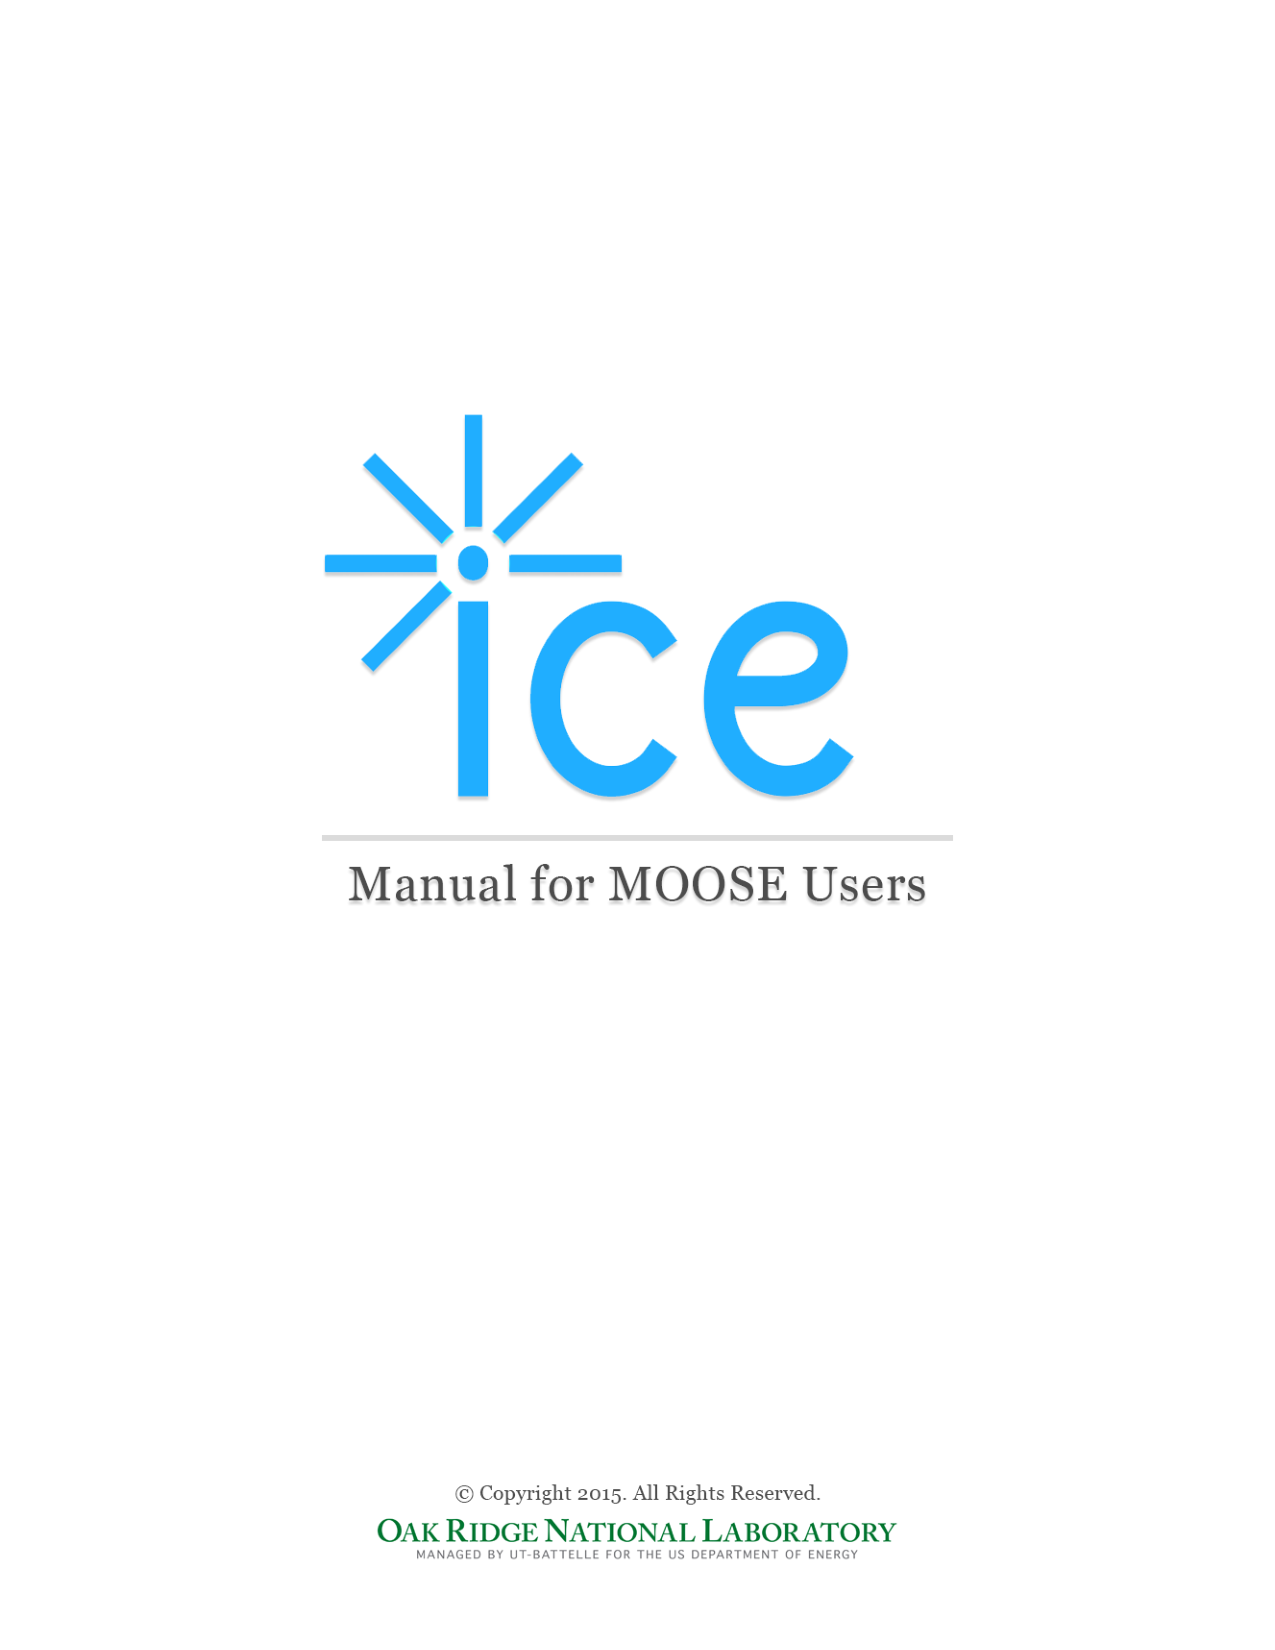
\includepdf{sections/ICEManual}
%Construct the title and author list
\title{ICE Manual for MOOSE Users} 
\author[a,b]{Jay Jay Billings, \thanks{Corresponding author.
Telephone:
+1 865 241 6308, Email: billingsjj@ornl.gov}} %, Twitter: @jayjaybillings}}
\author[a]{Alexander McCaskey, }
\author[a]{Anna Wojtowicz, }
\author[a]{Jordan H.\ Deyton}
\affil[a]{Oak Ridge National Laboratory PO Box 2008 MS 6173 Oak Ridge, TN 37831 USA}
\affil[b]{The Bredesen Center for Interdisciplinary Research and Education, The University of Tennessee, Knoxville, TN 37996 USA}
\end{titlepage}
\maketitle

\tableofcontents

%Input all of the sections of the paper
\chapter{Using MOOSE with ICE}
\label{sec:usingMoose}
\section{Introduction}\label{introduction}

This document is designed to outline the basic steps of setting up and
using the MOOSE plug-ins in ICE. ICE currently supports four MOOSE-based
applications: MARMOT, BISON, RELAP-7 and RAVEN. Although this tutorial
was created with BISON in mind, the steps for using ICE with MARMOT,
RELAP-7 and RAVEN are the same.

There are two different tasks for the input generation and launching of
MOOSE products within ICE:

\begin{itemize}
\itemsep1pt\parskip0pt\parsep0pt
\item
  \textbf{MOOSE Model Builder} - Generates a custom input file necessary
  to launch a MARMOT, BISON, RELAP-7 or RAVEN job.
\item
  \textbf{MOOSE Launcher} - Initiates the MARMOT, BISON, RELAP-7 or
  RAVEN codes to run on a local or remote system using the files
  generated from the \emph{MOOSE Model Builder}. Also includes the
  option to run a custom MOOSE-based application.
\end{itemize}

Any problems should be reported directly to the ICE team by sending an
email to the project list,
\texttt{ice-dev\ \textless{}at\textgreater{}\ eclipse.org}, or following
the instructions to report bugs on our Bugzilla site
\url{https://bugs.eclipse.org/bugs/describecomponents.cgi?product=Ice}.

\begin{center}\rule{0.5\linewidth}{\linethickness}\end{center}

\subsection{Installation and
Configuration}\label{installation-and-configuration}

Follow the instructions in the Getting ICE article at \url{wiki.eclipse.org/ICE} article
to download and install the latest version of ICE on your system.

\subsection{Prerequisites}\label{prerequisites}

You should have the MOOSE environment installed, either your local or
remote machine. Instructions for installing MOOSE can be found
\url{http://mooseframework.org/getting-started/}.

Additionally, you should have MARMOT, BISON, RELAP-7 or RAVEN compiled
and ready to run. Contact the development teams of these projects on the
rules and regulations for obtaining these codes.

\section{MOOSE Perspective}\label{moose-perspective}

ICE supports numerous plugins from different areas of science, and as a
result it can sometimes be difficult for new users to make sense of all
the different windows, panels and tabs in the workbench. To address this
issue for MOOSE users, ICE now includes a \emph{MOOSE Perspective} which
pares down UI components to only those that are necessary for
MOOSE-based plugins.

To access the \emph{MOOSE Perspective}, use the the ICE toolbar at the
top and navigate to:

\emph{Window} \textgreater{} \emph{Open Perspective} \textgreater{}
\emph{Other...}

Select \emph{MOOSE} in the window that pops up and click \emph{OK}.
Alternatively, you can also access the same pop-up menu by clicking the
\emph{Open Perspective} button in the upper right-hand corner of the ICE
workbench.

\begin{figure}[htbp]
\centering
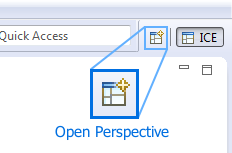
\includegraphics{figures/ICE_OpenPerspective.png}
\caption{The Open Perspective button in ICE for switching to other perspectives such as MOOSE or Visualization.}
\end{figure}

Once the MOOSE Perspective opens, you should notice the workbench now
contains fewer UI components, and resembles something like this:

\begin{figure}[htbp]
\centering
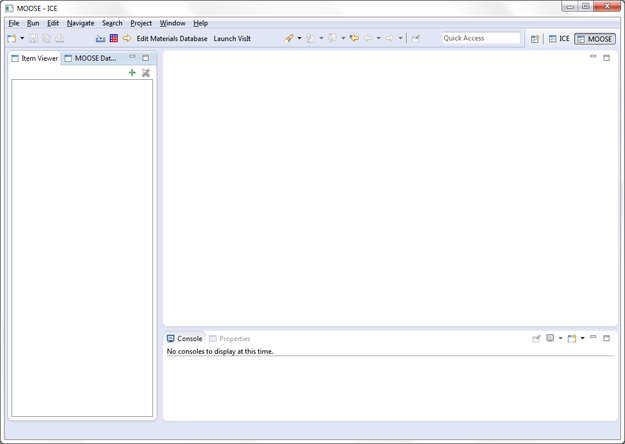
\includegraphics[width=\textwidth]{figures/ICE_MOOSEPerspective.png}
\caption{The MOOSE Perspective in ICE.}
\end{figure}

While it's not necessary to switch to the MOOSE Perspective to use
MOOSE-based plugins, it has been included for convenience.

\begin{center}\rule{0.5\linewidth}{\linethickness}\end{center}

\subsection{Generating YAML and Action Syntax
Files}\label{generating-yaml-and-action-syntax-files}

Like any MOOSE-based GUI, ICE relies on generated YAML and action syntax
files to specify the rules of creating input files. To simplify this
task, ICE includes a utility that will generate these files (either
locally or remotely), clean them up, and place them in the appropriate
local directory for ICE to use. All that is required of the user is to
specify where and on which machine their MOOSE codes are installed.

This task must be completed at least once for every installation of ICE
before the \emph{MOOSE Model Builder} can be used. It's also a good idea
to periodically re-run this utility to keep ICE's YAML and action syntax
files in sync with any updates to your MOOSE-based codes.

To use this utility, begin by clicking the document-like button in the
ICE toolbar:

\begin{figure}[htbp]
\centering
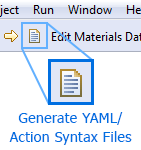
\includegraphics{figures/ICE_YAMLGeneratorButton.png}
\caption{The Generate YAML/Action Syntax Files button in the ICE Toolbar.}
\end{figure}

This will prompt a wizard to pop up requiring a few pieces of
information:

\begin{itemize}
\itemsep1pt\parskip0pt\parsep0pt
\item
  \textbf{Hostname}\\This can be a local or remote machine.
\item
  \textbf{Execution Path}\\Enter the fully-qualified path to the
  ``trunk'' directory of your machine's MOOSE installation. For example,
  if I have BISON on a machine with the following structure:

\begin{verbatim}
/home/user/trunk/bison/bison-opt
\end{verbatim}

  I would set the execution path in ICE to be:

\begin{verbatim}
/home/user/trunk
\end{verbatim}

  If you are launching on a remote machine, also be sure that you have
  appropriate privileges for the execution path.\\
\item
  \textbf{Login Credentials}\\Your username and password (if required)
  on the host machine.
\end{itemize}

Once you have filled out the information, click \emph{Finish}. This will
launch a script on your designated machine that checks which MOOSE-based
codes you have installed, generates the appropriate files, removes any
extraneous header/footer text, and places them in your

\begin{verbatim}
/home/user/ICEFiles/default/MOOSE
\end{verbatim}

directory where ICE can reference them later.

\begin{center}\rule{0.5\linewidth}{\linethickness}\end{center}

\subsection{Creating Input}\label{creating-input}

To create an input file for a MOOSE problem, there are two ways you can
get started: \textbf{creating an input file from scratch}, or
\textbf{importing an already existing file to modify}.

\subsubsection{Creating an Item}\label{creating-an-item}

If you'd like to start from scratch, begin by clicking the green +
button in the \emph{Item Viewer}, located on the left-hand side of the
ICE workbench.

\begin{figure}[htbp]
\centering
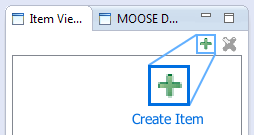
\includegraphics{figures/ICE_CreateItem.png}
\caption{The Create Item button in the ICE Item Viewer toolbar. }
\end{figure}

This will prompt a window to pop up; select the \emph{MOOSE Model
Builder} Item, and click \emph{Finish}.

Alternatively, if you'd like to import an already existing \texttt{*.i}
file to modify, click the yellow item import arrow located at the top of
the ICE workbench.

\begin{figure}[htbp]
\centering
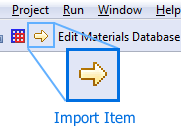
\includegraphics{figures/ICE_ImportItem.png}
\caption{The Import Item button in the ICE toolbar. }
\end{figure}

A wizard will pop up prompting you to specify two things: the
\texttt{*.i} file you'd like to import from your filesystem, and what
kind of \emph{Item} you'd like to import it into.

\begin{figure}[htbp]
\centering
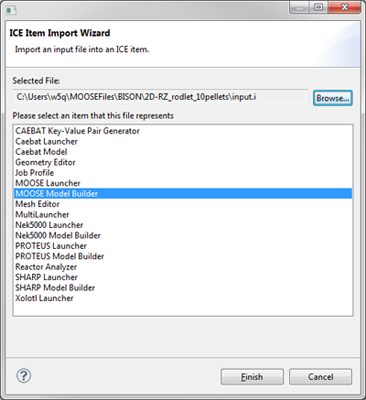
\includegraphics[scale=.8]{figures/ICE_ImportMOOSEModelBuilder.png}
\caption{The ICE Import Item Wizard. Select MOOSE Model Builder and a input file to import a fully populated MOOSE Model Item.}
\end{figure}

Use the \emph{Browse...} button to select your input file, and set the
item type to \emph{MOOSE Model Builder}. Click \emph{Finish} when you're
done and ICE will import the file data.

Regardless of how you decide to begin creating your input file, once the
\emph{MOOSE Model Builder} loads, you will see a workbench that looks
like the following. Make note of the three tabs highlighted: the \emph{Tree
View}, \emph{Mesh} and \emph{Properties} tabs, as we'll be using them
quite a bit in the following section.

\begin{figure}[htbp]
\centering
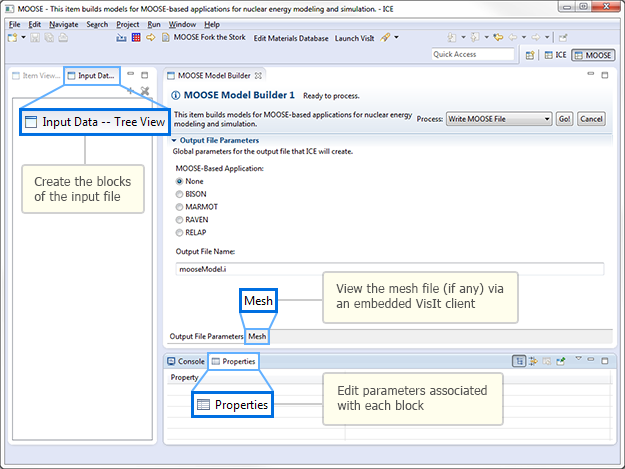
\includegraphics[width=\textwidth]{figures/ICE_MOOSEModelBuilder.png}
\caption{The MOOSE Model Builder, blank with no mesh selected.}
\end{figure}

\subsubsection{Constructing the Tree}\label{constructing-the-tree}

Before be begin constructing our problem, the first order of business is
to specify which MOOSE application we're defining a problem for. Using
the radio buttons in the main \emph{MOOSE Model Builder} tab, select one
of the options; in this example, we'll be creating a BISON problem.

\begin{figure}[htbp]
\centering
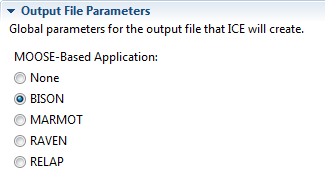
\includegraphics{figures/ICE_SelectMOOSEApp.png}
\caption{The MOOSE App Selection Widget. Select which MOOSE App's YAML tree to display}
\end{figure}

Once you've made a selection, it must be applied by saving the form.
Save by clicking the floppy-disk save icon (or \emph{Ctrl}+\emph{S}).

\begin{figure}[htbp]
\centering
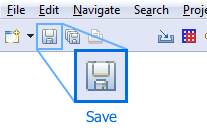
\includegraphics{figures/ICE_SaveButton.png}
\caption{The ICE Item Save button in the ICE toolbar.}
\end{figure}

At this point, a fully loaded set of blocks should appear in the
\emph{Tree View}. If you imported your data from an already existing
file, you'll notice the data has been loaded into any blocks that are
checked off. If you started from scratch, none of the blocks will be
checked off yet.

\begin{figure}[htbp]
\centering
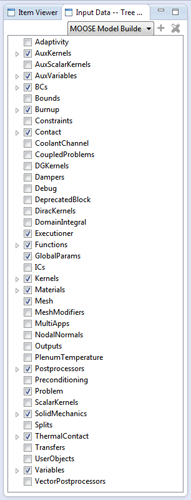
\includegraphics[scale=.9]{figures/ICE_LoadedMOOSETree.png}
\caption{The view of a fully loaded MOOSE input file tree.}
\end{figure}

We're now ready to begin using the \emph{Tree View} to add, delete and
modify blocks.

\paragraph{Expanding and Collapsing
Subblocks}\label{expanding-and-collapsing-subblocks}

If you imported data from an already existing input file, you will
likely notice some block names with a small arrow next to them. This
indicates that the block contains subblock structures beneath it. To
access these subblocks, simply click the small arrow and the subblocks
will expand. Clicking this arrow again will collapse the subblocks.

\begin{figure}[htbp]
\centering
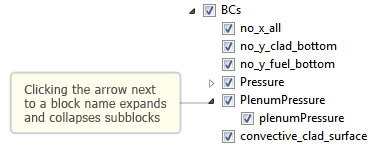
\includegraphics[scale=.8]{figures/ICE_MOOSEBlockExpand.png}
\caption{You can expand the nodes that have corresponding children in the input file.}
\end{figure}

\paragraph{Adding and Deleting Blocks}\label{adding-and-deleting-blocks}

If you'd like to add a subblock, first select the parent block you'd
like to add it to. Next, click the green + button located at the top
right-hand corner of the \emph{Tree View}. Alternatively, you can also
right-click the parent block, and select \emph{Add Child} from the
context menu that appears.

\begin{figure}[htbp]
\centering
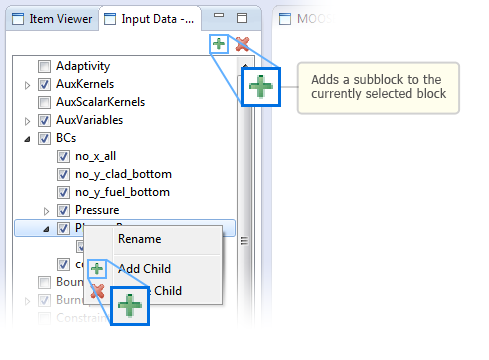
\includegraphics[scale=.6]{figures/ICE_MOOSEAddBlock.png}
\caption{Add a child block to the top-level MOOSE input file tree by selecting the green add button. }
\end{figure}

Doing this will prompt a pop-up dialog to appear. This dialog contains a
list of all possible subblocks that can be added, according to rules
outlined in the YAML files generated earlier. Each block that appears in
the list has its own unique set of parameters, with the exception of
\texttt{BlankBlocks}, which are---as their name suggests---blocks that
are totally devoid of any data.

\begin{figure}[htbp]
\centering
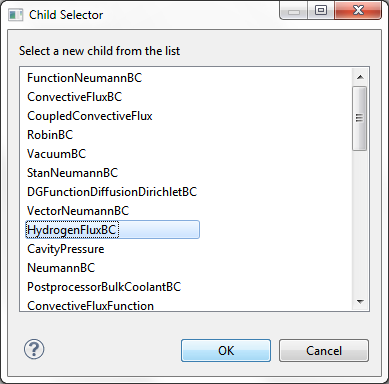
\includegraphics[scale=.85]{figures/ICE_MOOSESubblockList.png}
\caption{View of the possible children that can be selected for a BC block. Select one to add it to the tree.}
\end{figure}

Once you've selected a subblock to add, click \emph{OK}, and it will be
added in the \emph{Tree View}. Use the arrow next to the parent block to
expand/collapse the list of subblocks.

Similarly, to delete a block, select the particular block you'd like to
remove, and click the red ``x'' button located at the top right-hand
corner of the \emph{Tree View}. You can also delete a block by
right-clicking on it and selecting \emph{Delete Child} from the pop-up
context menu.

\begin{figure}[htbp]
\centering
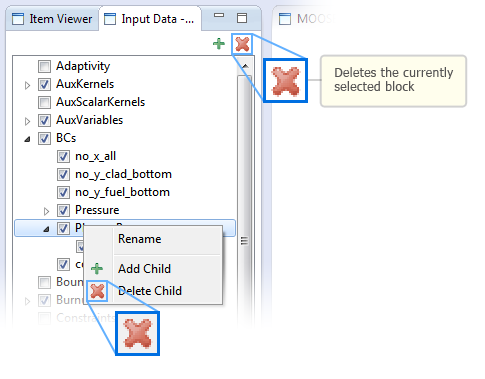
\includegraphics[scale=.6]{figures/ICE_MOOSEDeleteBlock.png}
\caption{Delete a child block by selecting the red delete button.}
\end{figure}

If the red ``x'' button is greyed-out for a particular block, this means
that deletion has been disabled. This is true for all top-level blocks.

\paragraph{Renaming Blocks}\label{renaming-blocks}

To rename a block, right-click on the block in question and select
\emph{Rename} from the context menu that appears. If the renaming option
is greyed-out from the context menu, this means that renaming has been
disabled for this block. Once again, this is true for all top-level
blocks.

\subsubsection{Editing Parameters}\label{editing-parameters}

Each block has a set of parameters associated to it. The default list of
parameters for each block is drawn from the YAML file that was generated
earlier. To add, remove or modify parameters associated to a block,
first select a block from the \emph{Tree View}. A table of parameters
will then appear in the \emph{Properties} tab referenced earlier.

The parameters table displays a parameter name, value and the option for
an in-line comment, which can all be edited directly in this table. When
written out to file, each parameter will be written to one line in the
form:

\begin{verbatim}
name = value     # comment
\end{verbatim}

Additional parameters can be added by clicking the + button to the
right of the parameter table; parameters can be similarly deleted by
clicking the "-" icon.

\begin{figure}[htbp]
\centering
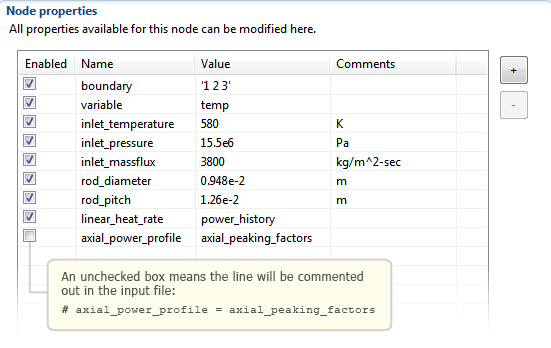
\includegraphics[width=\textwidth]{figures/ICE_MOOSEBlockParameters.png}
\caption{Clicking on a block in the MOOSE tree will display that block's set of edittable properties.}
\end{figure}

Next to each parameter row, you'll also notice an \emph{Enabled}
checkbox. Toggling this option on means that the parameter associated to
it will be written out normally in the file created. Toggling this
option off will cause the entire line to be commented out, and thus,
won't be used during the problem runtime.

Note that if you created a \emph{MOOSE Model Builder} by importing data
from an already existing input file, ICE automatically parses any
in-line comments or commented out lines (non-sensitive to leading
whitespaces). This will be reflected in the \emph{Enabled} and
\emph{Comment} columns of the parameters table.

Lastly, some blocks contain a special \texttt{type} parameter, such as
the \texttt{Executioner} block, which affects the list of parameters
associated to the block. In these special instances, an additional
drop-down menu will appear in the \emph{Property} tab, above the
parameters table.

\begin{figure}[htbp]
\centering
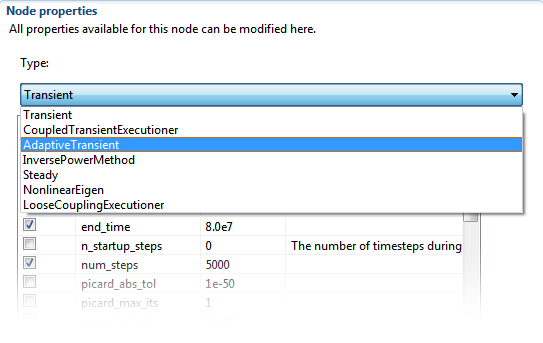
\includegraphics[width=\textwidth]{figures/ICE_MOOSEAdaptiveType.png}
\caption{Some blocks have an associated adaptive type, to change that type just select it from the dropdown at the top of the Properties view.}
\end{figure}

By setting the \texttt{type} of the block ICE automatically repopulates
the parameter table according to the rules defined by the YAML
specification.

\subsubsection{Viewing the Mesh File}\label{viewing-the-mesh-file}

If your MOOSE problem uses a mesh file, it can be viewed in an
interactive embedded VisIt client. More information about how to
correctly configure a VisIt session in ICE can be found in the
documentation in the \href{ICE_Embedded_Visualizations\#VisIt}{embedded
VisIt visualizations in ICE} following this section on using MOOSE.

To begin, make sure your \texttt{Mesh} block contains a parameter named
\texttt{file} by clicking on the \texttt{Mesh} block in the MOOSE tree
and examining its parameters in the \emph{Properties View}. The
\texttt{file} parameter should be set to the name of a \texttt{*.e} file
located in your
\texttt{/home/\textless{}user\textgreater{}/ICEFiles/default} directory.
You can either manually place the mesh file in that folder or import it
using the import button in ICE's main toolbar. If you need to add a
\texttt{file} parameter, do so now, and then save the form by clicking
the floppy-disk save icon (or \emph{Ctrl}+\emph{S}).

\begin{figure}[htbp]
\centering
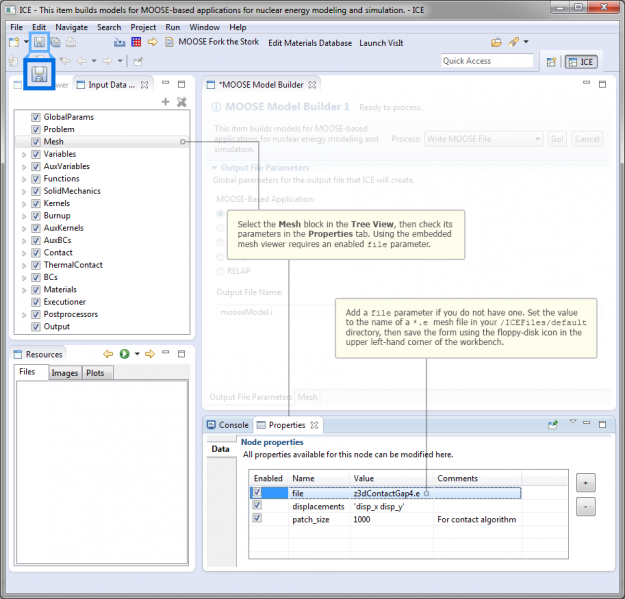
\includegraphics[width=\textwidth]{figures/ICE_MOOSE_Mesh-View-1.png}
\caption{The specialized MOOSE Model Mesh view. }
\end{figure}

When you save the MOOSE Model, ICE will attempt to load the file
specified by the \texttt{Mesh} block's \texttt{file} parameter as a
\emph{Resource}. To view the mesh, open the \emph{MOOSE Model Builder}'s
\emph{Mesh} tab, then double-click the mesh file \emph{Resource} in the
\emph{Resources View}. If the file can be read by one of ICE's
\emph{Visualization Services}, e.g., VisIt, the first available mesh in
the file will be opened in the \emph{Mesh} tab's \emph{Resource Page}.

\begin{figure}[htbp]
\centering
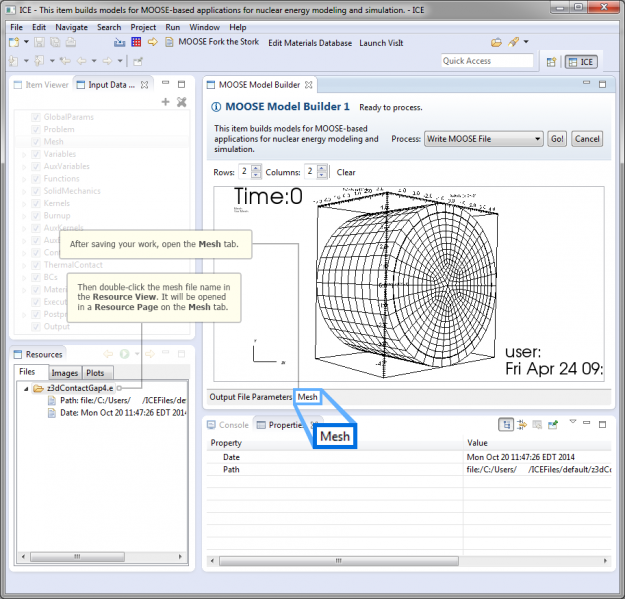
\includegraphics[width=\textwidth]{figures/ICE_MOOSE_Mesh-View-2.png}
\caption{The MOOSE Mesh View with selected mesh file displayed in the MOOSE Model Builder Mesh tab. }
\end{figure}

For more information about embedded visualizations like this or about
ICE \emph{Resources} and \emph{Resource Pages}, please see the
documentation in the \href{ICE_Embedded_Visualizations}{embedded
visualizations in ICE} section following this section on using MOOSE.

\subsubsection{Viewing the 3D Plant (RELAP-7
only)}\label{viewing-the-3d-plant-relap-7-only}

For RELAP-7 problems, ICE includes an interactive 3D \emph{Plant View}
to visualize the physical representation of the problem. To access the
\emph{Plant View}, click the \emph{Plant View} tab located at the bottom
of the main \emph{MOOSE Model Builder} panel.

\begin{figure}[htbp]
\centering
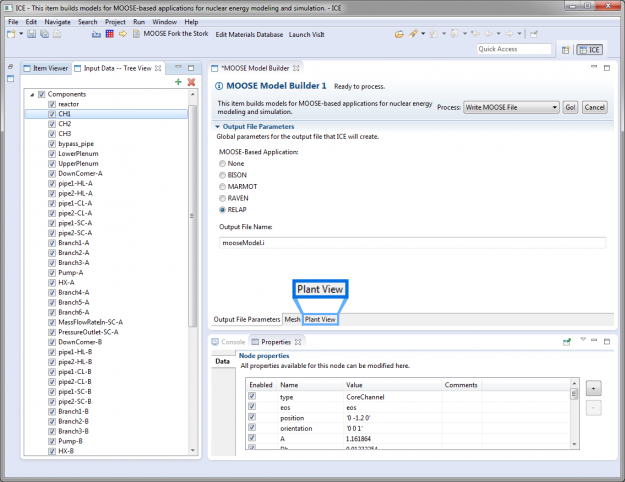
\includegraphics[width=\textwidth]{figures/ICE_MOOSEPlantViewTab.png}
\caption{If this is a RELAP-7 model, ICE displays a custom Plant-View tab.}
\end{figure}

This view draws data from the \texttt{Components} block in the
\emph{Tree View}; if you have valid components in the
\texttt{Components} block, then they should begin rendering now. Before
we go on, there are a few things to note about using the \emph{Plant
View}. First, only components that are currently enabled in the
\emph{Tree View} (i.e. have a checkmark) are rendered. This way,
components can easily be turned on and off without having to delete them
entirely. And secondly, the \emph{Plant View} updates in real time; any
changes that you make to components in the \emph{Tree View} will be
reflected immediately such as adding, removing, re-positioning or
re-orienting components.

\begin{figure}[htbp]
\centering
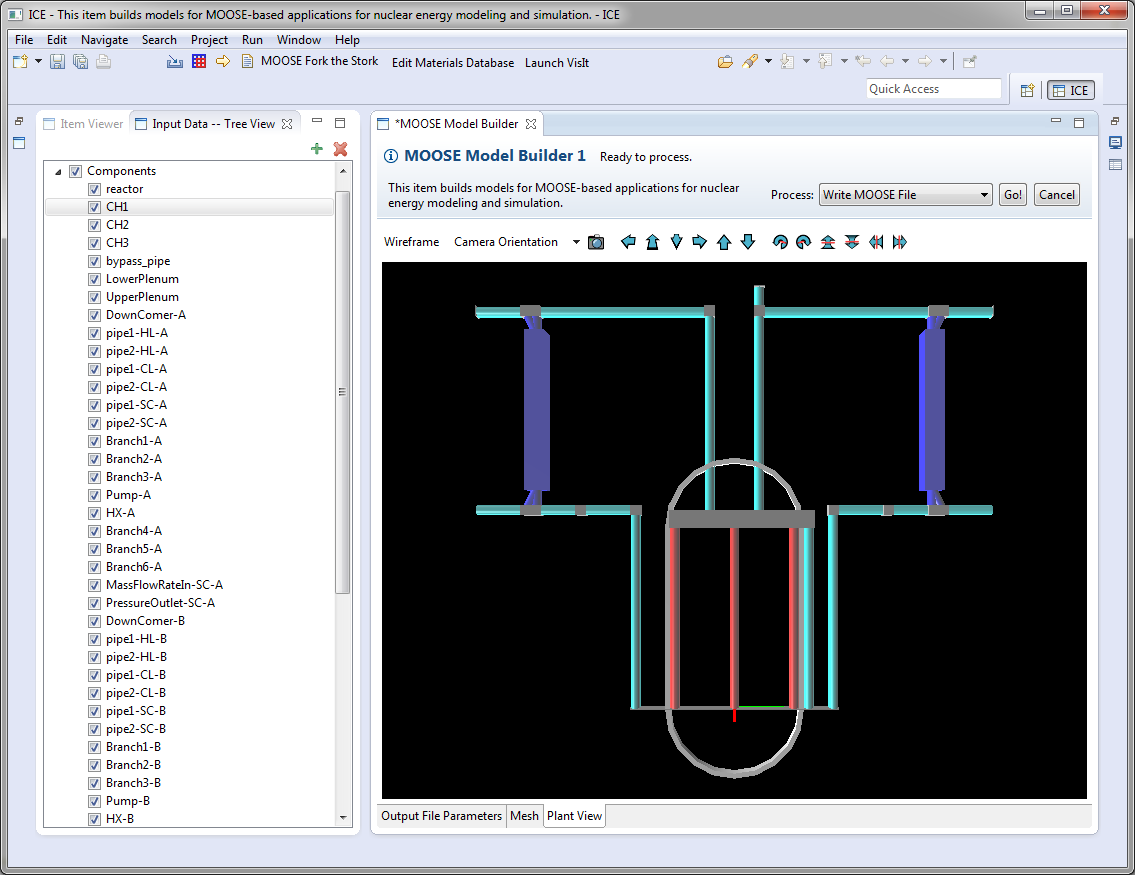
\includegraphics[width=\textwidth]{figures/ICE_MOOSEPlantView.png}
\caption{The ICE RELAP-7 Plant-View}
\end{figure}

Once your plant components have rendered, you can move around the 3D
space by using the arrow buttons in the toolbar above the viewing window
(hover over the button for a description of what it does), or by using
the following keyboard controls:

\begin{longtable}[c]{@{}llll@{}}
\caption{Camera Keyboard Controls}\tabularnewline
\toprule
Movement & Key & Rotation & Key\tabularnewline
\midrule
\endfirsthead
\toprule
Movement & Key & Rotation & Key\tabularnewline
\midrule
\endhead
Left & A & Roll right & Q\tabularnewline
Right & D & Roll left & E\tabularnewline
Up & C & Pivot left* & ←\tabularnewline
Down & Space & Pivot right* & →\tabularnewline
Forward & W & Pivot up* & ↑\tabularnewline
Backward & S & Pivot down* & ↓\tabularnewline
\bottomrule
\end{longtable}

* The camera viewing-angle can also be pivoted by left-clicking and
dragging

Lastly, the \emph{Plant View} has 3 other tools located in the toolbar
above the 3D viewing window, to the left of the movement/rotation
buttons.

\newpage

\begin{figure}[htbp]
\centering
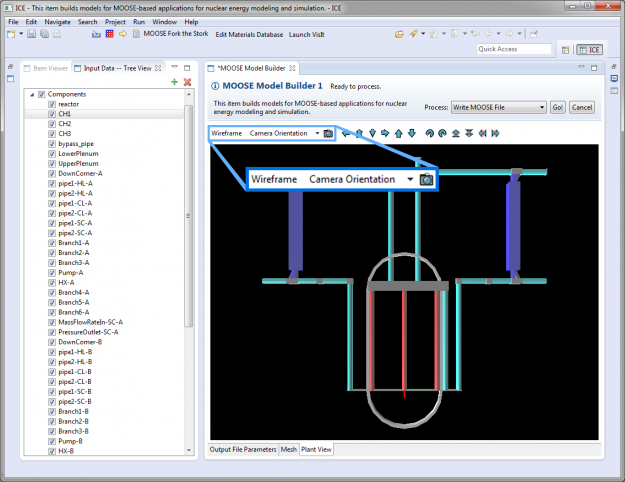
\includegraphics[width=\textwidth]{figures/ICE_MOOSEPlantViewTools.png}
\caption{A view of the ICE Plant-View controls. }
\end{figure}

\begin{itemize}
\itemsep1pt\parskip0pt\parsep0pt
\item
  \textbf{Wireframe} - Clicking this will toggle the plant's wireframe
  on and off; this allows you see how the meshes for the rendering
  engine are
  constructed.\\[2\baselineskip]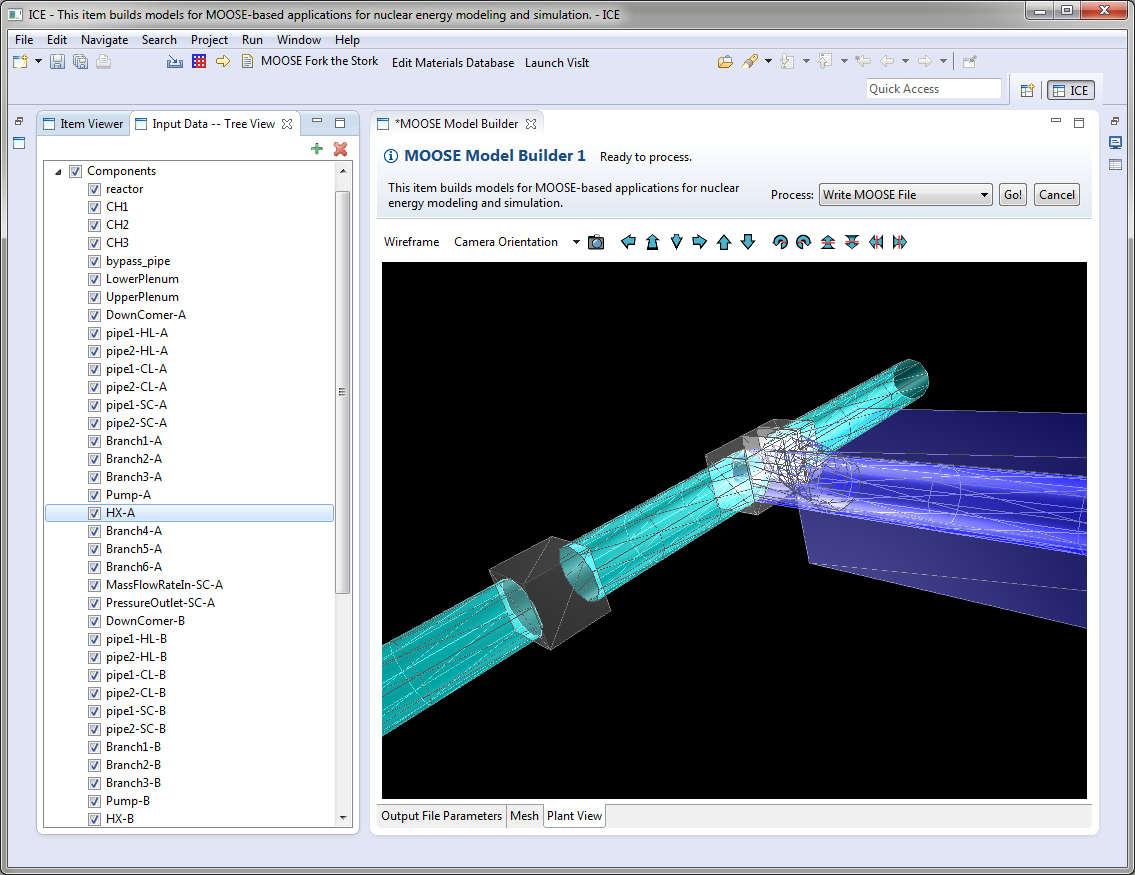
\includegraphics[width=.90\textwidth]{figures/ICE_MOOSEPlantViewWireframe.png}\\[2\baselineskip]In
  certain cases, this may be useful for verifying the plant model before
  running a simulation. For instance, pipe components in RELAP-7 have a
  property called ``n\_elems'' representing the number of cylindrical
  cross-section slices along the pipe's length. By switching to
  wireframe mode, the user can see the same number of cylindrical
  sections stacked together that represent the pipe's physical
  construction.
\end{itemize}

\begin{itemize}
\itemsep1pt\parskip0pt\parsep0pt
\item
  \textbf{Camera Orientation} - You can re-orient the rendering engine's
  default camera view by clicking on the \emph{Camera Orientation}
  button. The default orientation---YZ---is the standard \emph{} physics
  orientation with the Y axis increasing to the right, the Z axis
  increasing upwards, and the camera looking at the YZ-plane along the
  positive X axis.\\[2\baselineskip]In the same ``Camera Orientation''
  menu, we provide two alternative default orientations: the XY
  orientation shows the XY-plane from along the positive Z axis, and the
  ZX orientation shows the ZX-plane from along the positive Y axis.
  Selecting \emph{Reset to current default} will snap the camera back to
  the origin view should you ever get lost.
\end{itemize}

\begin{itemize}
\itemsep1pt\parskip0pt\parsep0pt
\item
  \textbf{(\emph{Camera Icon} - Save Image)} - Clicking this will prompt
  a pop-up window to save a \texttt{.png} image of the current
  \emph{Plant View} to your local filesystem.
\end{itemize}

\subsubsection{Creating the File}\label{creating-the-file}

Once you have edited your blocks and associated parameters to your
liking, the last step is to write them to file.

Any top-level block in the \emph{Tree View} with a checkmark next to it
will be written to file, and any top-level blocks without a checkmark
will not. Similarly, any \emph{sub}-blocks with a checkmark will also
written to file, however, any sub-blocks \emph{without} a checkmark will
still be written to file but commented out. Ensure that you've correctly
checked/unchecked all the necessary blocks. Save your work by clicking
the floppy-disk save icon (or \emph{Ctrl}+\emph{S}).

In the main \emph{MOOSE Model Builder} tab, specify the name of the file
you'd like to write in the \emph{Output File Name} field. Next, in the
top right-hand corner, set the \emph{Process} drop-down menu to ``Write
MOOSE File'', and click the \emph{Go!} button.

\begin{figure}[htbp]
\centering
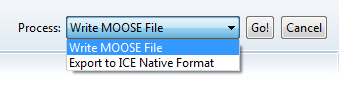
\includegraphics[width=\textwidth]{figures/ICE_MOOSEWriteFile.png}
\caption{The Write File Entry for specifying the name of the input file you'd like to write.}
\end{figure}

This will write the contents of your \emph{Tree View} to the specified
filename, and will be placed in your \texttt{/ICEFiles/default}
directory. If you wish to review the file before moving onto the next
section, you can do so by using the ICE toolbar and navigating to:

\emph{File} \textgreater{} \emph{Open File...}

\begin{center}\rule{0.5\linewidth}{\linethickness}\end{center}

\subsection{Launching a MOOSE Job}\label{launching-a-moose-job}

Once you've generated appropriate input files, launching a MOOSE job is
a relatively simple task.

To get started, click the green + button in the \emph{Item Viewer}
once more to create a new ICE Item.

\begin{figure}[htbp]
\centering
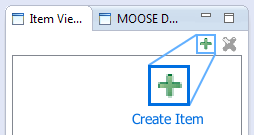
\includegraphics{figures/ICE_CreateItem.png}
\caption{The Create Item button in the ICE Item Viewer toolbar.}
\end{figure}

Select \emph{MOOSE Launcher} from the menu that pops up and click
\emph{Finish}.

A form will appear in the main ICE workbench area. This form contains
the information necessary for launching a MOOSE problem.

\begin{figure}[htbp]
\centering
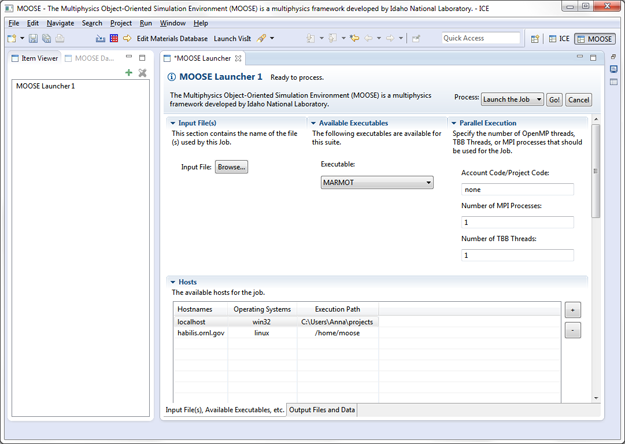
\includegraphics[width=\textwidth]{figures/ICE_MOOSELauncher.png}
\caption{The MOOSELauncher View. }
\end{figure}

\subsubsection{Selecting the Input
File(s)}\label{selecting-the-input-files}

From the \emph{Input File(s)} drop-down menu, select an appropriate
MOOSE input file. This drop-down menu displays all \texttt{*.i} files
that were in the \texttt{/ICEFiles/default} directory at the time the
\emph{MOOSE Launcher} was created. If you created your own input file in
the previous step using the \emph{MOOSE Model Builder}, this file should
appear in the list of available files.

If you'd like to use an input file not found in this list, click the
\emph{Browse...} button; a file browser will pop up for you to locate
the file you'd like to use. Once you've selected a file, it will be
imported into the \texttt{/ICEFiles/default} directory.

\begin{figure}[htbp]
\begin{center}
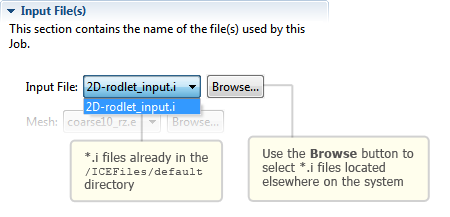
\includegraphics[scale=.6]{figures/ICE_MOOSEInputFiles.png}
\caption{Select the input file to launch with the specified MOOSE application. You can browse the file system for the input file if it is not located in your ICEFiles/default workspace.}
\end{center}
\end{figure}

At this time, the \emph{MOOSE Launcher} will scan the \texttt{*.i} file
for any references to additional files, such as a mesh, peaking factors,
power history, etc. If any additional file dependencies are found, the
\emph{MOOSE Launcher} will dynamically render additional file entries
for your to set in the same manner.

\subsubsection{Selecting the MOOSE
Product}\label{selecting-the-moose-product}

You will need to indicate which MOOSE-based application you'd like to
run. From the list of \emph{Available Executables}, simply select one of
the available applications.

\begin{figure}[htbp]
\centering
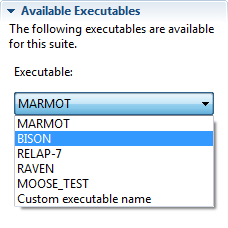
\includegraphics{figures/ICE_MOOSEAvailableExecutables.png}
\caption{A list of the available MOOSE applications to choose from.}
\end{figure}

If you'd like to launch a custom MOOSE application not listed, you also
have the option of doing so. Select \emph{Custom executable name} from
the drop-down menu, and enter your application's name in the text field
that appears.

\begin{figure}[htbp]
\centering
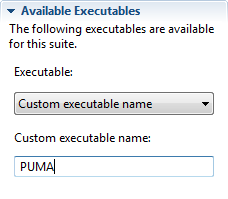
\includegraphics{figures/ICE_MOOSELauncherCustomExecutable.png}
\caption{You can now specify a custom executable!}
\end{figure}

If we were to use the example in Figure 1.27, ICE would attempt to launch an
executable called \texttt{PUMA-opt} (and not \texttt{puma-opt}). To
learn more about creating your own custom MOOSE-based applications in ICE, read
the \href{Developing MOOSE Applications with ICE}{Developing MOOSE
Applications with ICE} section of this tutorial document following this section on using MOOSE.

\subsubsection{Specifying a Hostmachine}\label{specifying-a-hostmachine}

From here, the next step is to tell ICE which machine your MOOSE code
will be run on, either locally or remotely. A list of hosts used at ORNL
is displayed by default, however, additional hosts can be added by
clicking the + button to the right of the \emph{Hosts} table.

\begin{figure}[htbp]
\centering
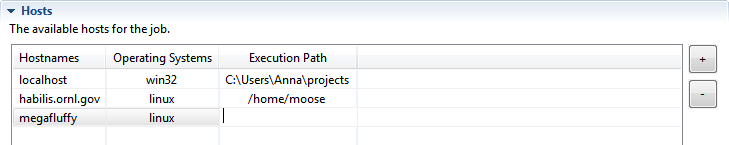
\includegraphics[width=\textwidth]{figures/ICE_MOOSEHostsTable.png}
\caption{The MOOSELauncher Hosts table. Specify the hosts that you'd like to launch the application on.}
\end{figure}

When adding hosts, set the \emph{Execution Path} to the trunk directory
of the machine's MOOSE installation. For example, if I'm launching BISON
on a machine with the follow structure:

\begin{verbatim}
/home/user/trunk/bison/bison-opt
\end{verbatim}

I would set the execution path in ICE to be:

\begin{verbatim}
/home/user/trunk
\end{verbatim}

If you are launching on a remote machine, also be sure that you have
appropriate privileges for the execution path.

\subsubsection{Setting Parallel Execution
(Optional)}\label{setting-parallel-execution-optional}

Optionally, if you'd like to take advantage of parallel processing, you
may specify the number of MPI process and/or Intel Thread Building Block
(TBB) threads.

\begin{figure}[htbp]
\centering
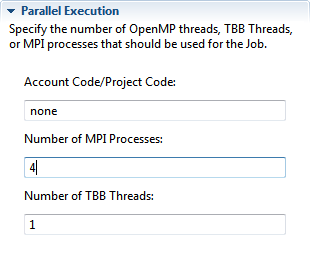
\includegraphics{figures/ICE_ParallelExecution.png}
\caption{You can specify how many MPI processes, OpenMP threads, or Intel TBB threads to use in your application launch.}
\end{figure}

To use multiple MPI processes, change the marked field to an integer
value anywhere between 1 and 10000. Note that \texttt{mpirun} must be
specified in the host machine's \texttt{PATH} variable. If you choose
not to change this field, the default value of 1 MPI process is used.

To use multiple TBB threads, change the marked field to an integer value
anywhere between 1 and 256. Note that the host machine must have Intel
TBB support. If you choose not to change this field, the default value
of 1 TBB thread is used.

\subsubsection{Launching the Problem}\label{launching-the-problem}

Once the input file(s), host, and any parallel execution options are
specified, save your settings. If you make any subsequent changes to the
\emph{MOOSE Launcher} form, you will have to re-apply them by saving the
form in the same way.

Lastly, use the \emph{Process} menu in the upper right-hand corner;
select the \emph{Launch the Job} task from the drop-down menu and click
the \emph{Go!} button.

\begin{figure}[htbp]
\centering
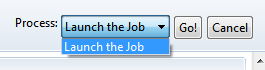
\includegraphics{figures/ICE_LaunchJob.png}
\caption{Select the Launch the Job action and click Go to launch your MOOSE application.}
\end{figure}

Depending on your host machine's configuration, you may be prompted for
login credentials.

You should shortly begin seeing the standard console output in ICE as
your problem begins to solve.

\chapter{Embedded Visualizations in ICE}
\label{sec:embeddedViz}

\section{Introduction}\label{introduction}

This document describes the embedded visualization capabilities
available in ICE. Embedded visualizations in ICE aim to provide users
with immediate yet simple visualization of simulation input and output
well within the simulation workflow. In other words, simulation input
and output can be visually verified or validated without leaving the
associated Model Builder or Job Launcher in ICE. For more advanced or
complex visualization tasks in ICE, please see the document on
\href{Visualizing Output with ICE}{Visualizing Output with ICE}.

\section{Resources and Resource
Pages}\label{resources-and-resource-pages}

ICE \emph{Items} may include any number of \emph{Resources}, which may
include any type of file like meshes, pictures, shell scripts,
\texttt{.csv} files, or even plain text files. For example, a
\emph{Model Builder}, which is used in ICE to configure simulation
input, may at some point include a plain text input file as well as
associated data files or meshes. Likewise, a \emph{Job Launcher}, which
actually launches the simulation, may produce any type of output data,
which may also include \texttt{.csv} files, binary files, or even more
mesh files.

Before proceeding, you should familiarize yourself with the
\emph{Resources View} (highlighted in blue on the left) and the idea of
a \emph{Resource Page} (highlighted in red, while its tab is highlighted
at the bottom) as shown in the image below.

\begin{figure}[htbp]
\centering
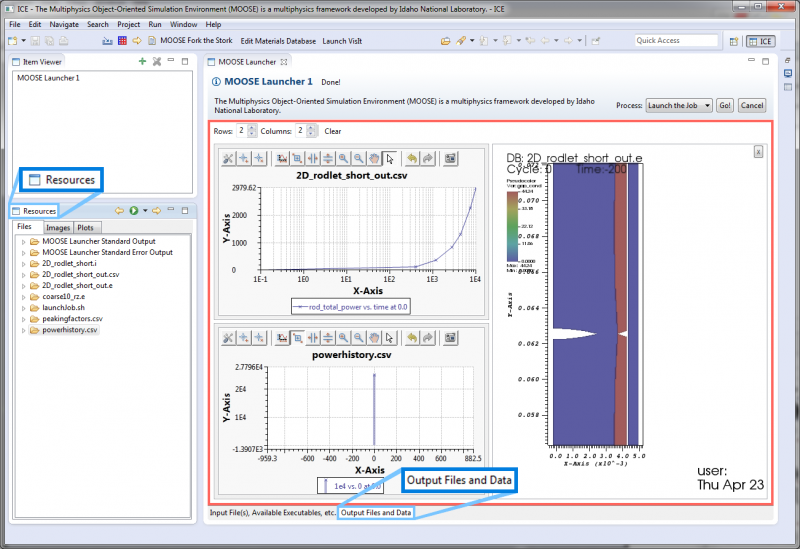
\includegraphics[width=\textwidth]{figures/ICE_Viz_ResourceViewPage.png}
\caption{The new ICE Resource View showing generated output files that can be visualized natively in the view. }
\end{figure}

\subsubsection{The Resources View}\label{the-resources-view}

Some \emph{Items} in ICE store references to these resources for easy
access to the user. In these cases, the resources are presented to the
user in the \emph{Resources View}, which is part of the default ICE
perspective.

The \emph{Resource View} is actually a tree, where each resource has its
own node. If you expand a resource node, it will reveal the underlying
file's path along with its date of last modification.

\subsubsection{Resource Pages}\label{resource-pages}

If an ICE \emph{Item} includes resources, it will have a designated tab
for showing those resources.

\begin{itemize}
\itemsep1pt\parskip0pt\parsep0pt
\item
  For \emph{Model Builders}, this tab could be named anything. For
  instance, in the \emph{MOOSE Model Builder}, the tab for viewing
  resources is called \emph{Mesh}.
\item
  For \emph{Job Launchers}, this tab will be named \emph{Output Files
  and Data}.
\end{itemize}

Click on the tab to open it and view the \emph{Item}'s \emph{Resource
Page}. Each \emph{Resource Page} is capable of showing plain text files
or embedded visualizations based on the selected resource's file type.

\subsubsection{Viewing a Resource}\label{viewing-a-resource}

To open a resource, go to the \emph{Resources View} and double-click its
item in the list of available resources. The way ICE handles this
selected resource depends on the following:

\begin{enumerate}
\itemsep1pt\parskip0pt\parsep0pt
\item
  If the file can be opened using one of the visualization services, it
  will be added to the active \emph{Resource Page}.
\item
  If the file can be opened using a plain text editor, it will be opened
  in a new \emph{Text Editor} in ICE.
\item
  If the file cannot be opened, the \emph{Resource Page} will attempt to
  render it through a browser widget. This handles some basic files like
  certain image types.
\item
  If the file cannot be opened in the browser, the browser will prompt
  you to save the file. In this case, you can either save it, or cancel
  and open the existing file at the location specified in the
  \emph{Resources View}.
\end{enumerate}

This document will not discuss the latter three situations any further.
The next sections will describe the embedded visualizations from the
first scenario.

\subsubsection{Controlling Embedded
Visualizations}\label{controlling-embedded-visualizations}

Each \emph{Resource Page} can display a number of embedded
visualizations at any time. Selected plots are displayed in a grid
defined by the \emph{Rows} and \emph{Columns} widgets in the toolbar
(highlighted in blue in the image below) near the top of the page,
although embedded plots will take up as much space as they can. The
default grid is two by two, although the number of rows and columns can
be changed at any time.

\begin{figure}[htbp]
\centering
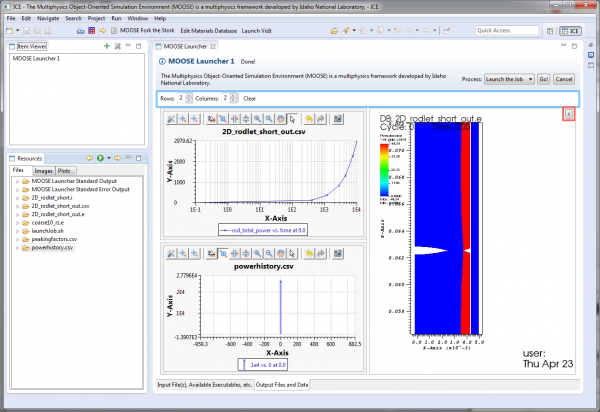
\includegraphics[width=\textwidth]{figures/ICE_Viz_Grid.png}
\caption{The Resource Page grid of plots can be modified through the rows/columns toggle buttons.}
\end{figure}

\paragraph{Adding Plots to the Grid}\label{adding-plots-to-the-grid}

To add a new plot to the grid, simply go to the \emph{Resources View}
and double-click the desired file that can be rendered by one of ICE's
visualization services. Note that the order in which plots appear in the
grid depend on the order in which they are added to the grid, with the
grid moving left-to-right, top-to-bottom.

\paragraph{Removing Plots from the
Grid}\label{removing-plots-from-the-grid}

To remove an individual plot, you have two choices:

\begin{enumerate}
\itemsep1pt\parskip0pt\parsep0pt
\item
  You can hover the mouse cursor over the plot, then click the ``X''
  button that appears (highlighted in red in the image above).
\item
  You can right-click somewhere inside the plot, then click
  \emph{Remove}.
\end{enumerate}

You can also remove all plots at once by clicking the \emph{Clear}
button in the \emph{Resource Page}'s toolbar. This is located next to
the widgets for controlling the size of the grid.

\paragraph{Right-click Menus}\label{right-click-menus}

Every plot drawn inside the \emph{Resource Page} includes a right-click
menu that provides the following basic options:

\begin{enumerate}
\itemsep1pt\parskip0pt\parsep0pt
\item
  \textbf{Remove} - Removes the plot from the \emph{Resource Page}
\item
  \textbf{Set Plot Type} - Provides nested sub-menus that let you set
  what is displayed in the plot.
\end{enumerate}

The contents of the \emph{Set Plot Type} sub-menu depends on both the
file and the visualization service used to plot it. Generally, you first
choose the plot \emph{category} from the first sub-menu and then a
\emph{type} from the category sub-menu.

Additional menu choices may be available depending on the visualization
service that provides the plot.

\section{Visualization Services}\label{visualization-services}

\subsubsection{VisIt}\label{visit}

\paragraph{Prerequisites}\label{prerequisites}

To use the embedded visualization service for \emph{VisIt}, ICE requires
a local installation of
\href{https://wci.llnl.gov/simulation/computer-codes/visit/}{VisIt}
(minimum version 2.8.2) developed by Lawrence Livermore National
Laboratory.

\paragraph{Preferences}\label{preferences}

\subparagraph{Getting to the
Preferences}\label{getting-to-the-preferences}

Using the \emph{VisIt} visualization service for viewing complex 2D or
3D mesh data requires little initial configuration. Assuming the
\hyperref[Prerequisites]{VisIt prerequisite} is installed, use the the
main menu bar at the top of the window and navigate to:

\emph{Window} \textgreater{} \emph{Preferences}

In the \emph{Preferences} dialog, navigate to:

\emph{Visualization} \textgreater{} \emph{VisIt} (highlighted in blue in
the image below)

\begin{figure}[htbp]
\centering
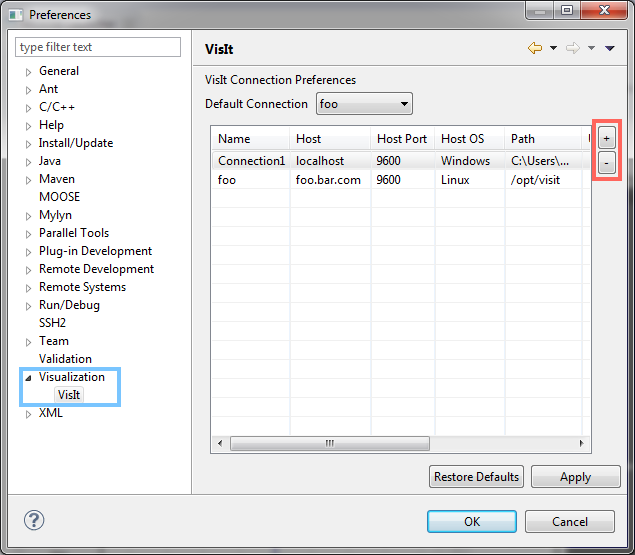
\includegraphics[width=\textwidth]{figures/ICE_Viz_VisIt_Preferences.png}
\caption{The new VisIt Preferences Page.}
\end{figure}

\subparagraph{Adding Connections}\label{adding-connections}

You will need to press the + button (highlighted above in red) to the
right of the table to add a new entry. Fill out the new row in the
table. Generally speaking, the default values are fine, but the
\emph{Path} will need to be updated to point to the folder containing
your VisIt executable. You can copy and paste the path into this field
and press \emph{Enter}.

\subparagraph{Setting the Default
Connection}\label{setting-the-default-connection}

Currently, only one connection to VisIt can be used at a time. If you
only have one configured connection, it is automatically selected as the
default. However, if you have multiple configured connections, you will
need to set the \emph{default} connection by choosing from the drop down
above the table.

\subparagraph{Removing Connections}\label{removing-connections}

To remove a connection, click on any cell in its row in the table, then
click the "-" button (highlighted above in red) on the right of the
table. You can select multiple connections by holding \emph{CTRL} while
you click them, then clicking the "-" button.

\subparagraph{Applying the Connection
Preferences}\label{applying-the-connection-preferences}

When you have finished updating your connection configurations for
VisIt, you can click \emph{OK} to apply the changes and close the
\emph{Preferences} dialog. Alternatively, you can apply the changes
immediately by clicking \emph{Apply}. It is then safe to close the
\emph{Preferences} dialog in any valid way, e.g., by clicking the
dialog's close button or by clicking \emph{Cancel}.

\paragraph{Opening a VisIt Plot}\label{opening-a-visit-plot}

The \emph{Resources View} will pass any ICE resources pointing to
\texttt{.e} (Exodus) or \texttt{.silo} files to the \emph{VisIt
Visualization Service}. If the visualization service is configured and
running and if the file is valid, then the \emph{Resource Page} will
open a view of the resource powered by the default VisIt connection, as
in the image of a battery mesh SILO file below.

An example VisIt plot embedded in a \emph{Model Builder} can be seen in Figure 2.4.

\begin{figure}[htbp]
\centering
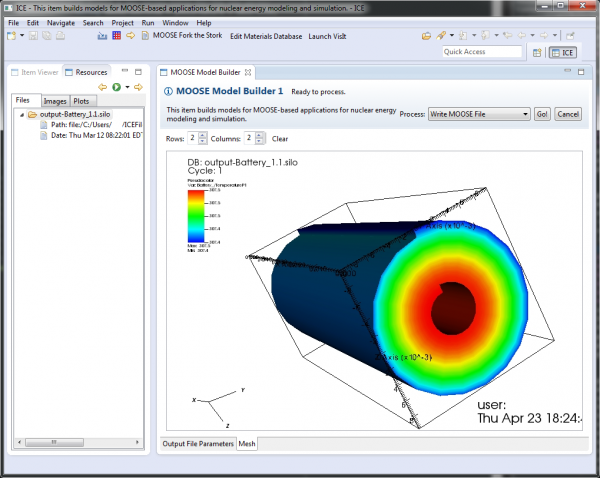
\includegraphics[width=\textwidth]{figures/ICE_Viz_VisIt.png}
\caption{An embedded VisIt plot in the MOOSE Model Builder. }
\end{figure}

The embedded VisIt view can be rotated by clicking and dragging and
zoomed in and out with the mouse wheel.

\paragraph{Right-click Menu}\label{right-click-menu}

The image below shows the context menu available when right-clicking
somewhere inside the VisIt view.

\begin{figure}[htbp]
\centering
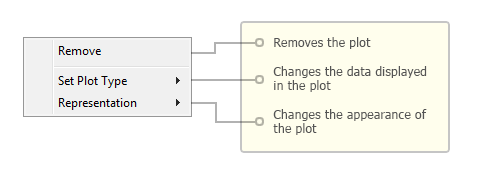
\includegraphics[scale=.6]{figures/ICE_Viz_VisIt-ContextMenu.png}
\caption{The embedded plot contains context-menu right-click functionality for modifying or deleting the plot.}
\end{figure}

The plot types available in the context menu depend on the data
available in the VisIt-compatible file. In the case of this SILO file,
the only plot categories are \emph{Meshes} and \emph{Scalars}.

The context menu also includes the ability to change how the VisIt plot
is rendered. The representations available depend on the current plot
type. A full list of supported ``representations'' is listed below for
each plot category.

\begin{itemize}
\itemsep1pt\parskip0pt\parsep0pt
\item
  Materials

  \begin{itemize}
  \itemsep1pt\parskip0pt\parsep0pt
  \item
    Boundary \emph{(default)}
  \item
    FilledBoundary
  \end{itemize}
\item
  Meshes

  \begin{itemize}
  \itemsep1pt\parskip0pt\parsep0pt
  \item
    Mesh \emph{(default)}
  \end{itemize}
\item
  Scalars

  \begin{itemize}
  \itemsep1pt\parskip0pt\parsep0pt
  \item
    Pseudocolor \emph{(default)}
  \item
    Contour
  \item
    Volume
  \end{itemize}
\item
  Vectors

  \begin{itemize}
  \itemsep1pt\parskip0pt\parsep0pt
  \item
    Vector \emph{(default)}
  \end{itemize}
\end{itemize}

\subsubsection{CSV}\label{csv}

\paragraph{Prerequisites}\label{prerequisites-1}

The embedded visualizations for \texttt{.csv} data require no additonal
software to be installed or any preference configuration.

\paragraph{Opening a CSV Plot}\label{opening-a-csv-plot}

The \emph{Resources View} will pass any ICE resources pointing to
\texttt{.csv} files to the \emph{CSV Visualization Service}. If the file
can be read by the \emph{CSV Visualization Service}, then the
\emph{Resource Page} will open a plot that contains the first available
series in the file.
An example CSV plot embedded in a \emph{Job Launcher} can be seen in Figure 2.6.

\begin{figure}[htbp]
\centering
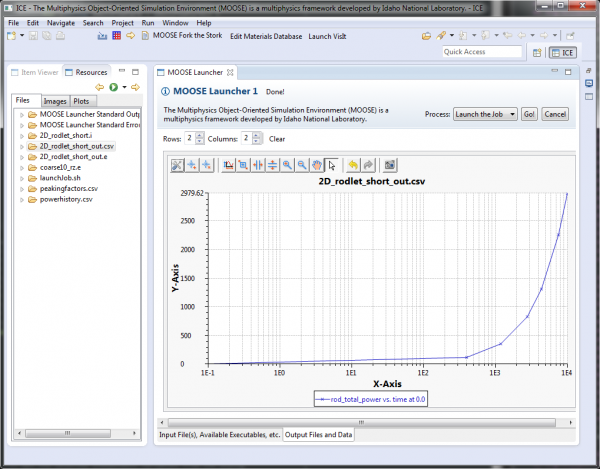
\includegraphics[width=\textwidth]{figures/ICE_Viz_CSV.png}
\caption{An embedded CSV plot in the MOOSE Launcher Resource Page, representing some MOOSE PostProcessor data.}
\end{figure}

The embedded CSV plot includes the same toolbar described in the the
standard features provided by the
\href{Visualizing_Output_with_ICE\#Plot_Toolbar}{\emph{CSV Plot Editor}
in the \emph{Visualization Perspective}} as well as a right-click menu
to modify the plot.

\paragraph{Right-click Menu}\label{right-click-menu-1}

The image below shows the context menu available when right-clicking
somewhere inside the CSV plot.

\begin{figure}[htbp]
\centering
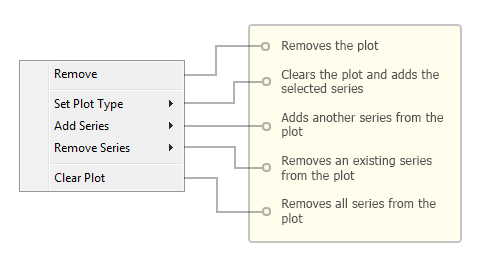
\includegraphics[width=\textwidth]{figures/ICE_Viz_CSV-ContextMenu.png}
\caption{The CSV context-menu. }
\end{figure}

By choosing a series from the \emph{Set Plot Type} sub-menu, you can
change what series is plotted. This will clear any existing series from
the plot and add the selected series.

To add more series to the plot, choose a series from the \emph{Add
Series} sub-menu.

To remove a plotted series, choose one of the existing series from the
\emph{Remove Series} sub-menu. This sub-menu will be disabled if there
are no series to remove.

To clear all series from the plot, click \emph{Clear Plot} at the bottom
of the menu.

\chapter{Visualizing Output in ICE}
\label{sec:visOutput}
Currently, ICE features two plugins for visualizing and plotting
simulation output data:

\begin{itemize}
\itemsep1pt\parskip0pt\parsep0pt
\item
  \textbf{VisIt Tools} - An interactive 3D visualization tool for
  rendering meshes, scalar plots, contour plots, and more.
\end{itemize}

\begin{itemize}
\itemsep1pt\parskip0pt\parsep0pt
\item
  \textbf{CSV Plotting Tools} - A customizable, 2D data plotting utility
  for data from \texttt{.csv} files.
\end{itemize}


\begin{figure}[htbp]
\centering
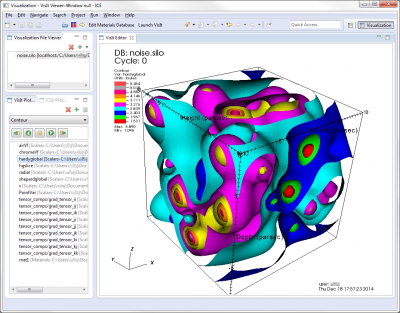
\includegraphics[width=\textwidth]{figures/ICE_VisIt.png}
\caption{A contour plot shown in the ICE VisIt Editor. }
\end{figure}

\begin{figure}[htbp]
\centering
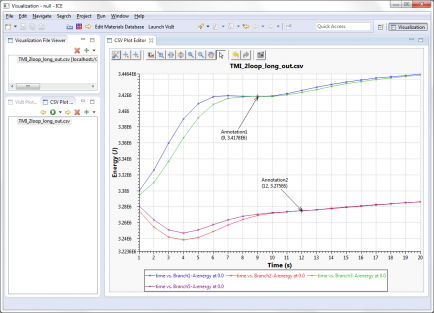
\includegraphics[width=\textwidth]{figures/ICE_CSVPlotter.png}
\caption{The ICE CSV Plot Editor showing MOOSE PostProcessor data.}
\end{figure}
\newpage
%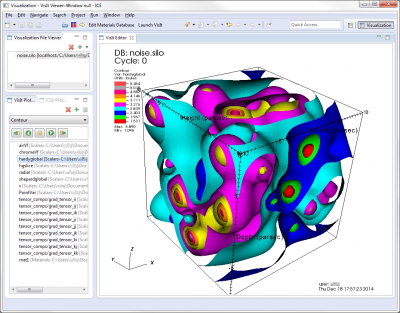
\includegraphics{figures/ICE_VisIt.png} 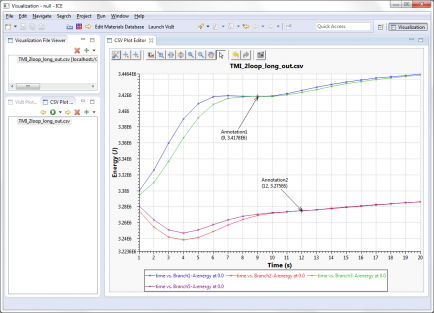
\includegraphics{figures/ICE_CSVPlotter.png}

\section{Installation and
Configuration}\label{installation-and-configuration}

\subsection{Prerequisites}\label{prerequisites}

To use the \emph{VisIt Tools}, ICE requires the installation of
\href{https://wci.llnl.gov/simulation/computer-codes/visit/}{VisIt}
(minimum version 2.8.2) developed by Lawrence Livermore National
Laboratory, either locally or on a remote machine.

The \emph{CSV Plotting Tools} require no additonal software to be
installed.

\subsection{Visualization
Perspective}\label{visualization-perspective}

To use ICE's visualization tools, you first must switch to the
\emph{Visualization Perspective}. This perspective includes various UI
components necessary for visualization that are not exposed in the
default ICE perspective. To access the \emph{Visualization Perspective},
use the the main menu bar at the top of the window and navigate to:

\emph{Window} \textgreater{} \emph{Open Perspective} \textgreater{}
\emph{Other}...

Select \emph{Visualization} in the dialog that pops up and click
\emph{OK}. Alternatively, you can also access the same pop-up dialog by
clicking the \emph{Open Perspective} button in the main toolbar in the
upper right-hand corner of the ICE workbench.

\begin{figure}[htbp]
\centering
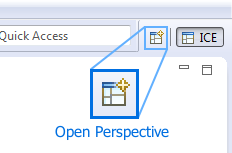
\includegraphics{figures/ICE_OpenPerspective.png}
\caption{The Open Perspective button for switching to another perspective, like in this case, the Visualization Perspective.}
\end{figure}

Once the \emph{Visualization Perspective} opens, you should notice the
workbench contains some new UI components. Make note of the following
panels, as we will be referring to them in the following sections.

\begin{figure}[htbp]
\centering
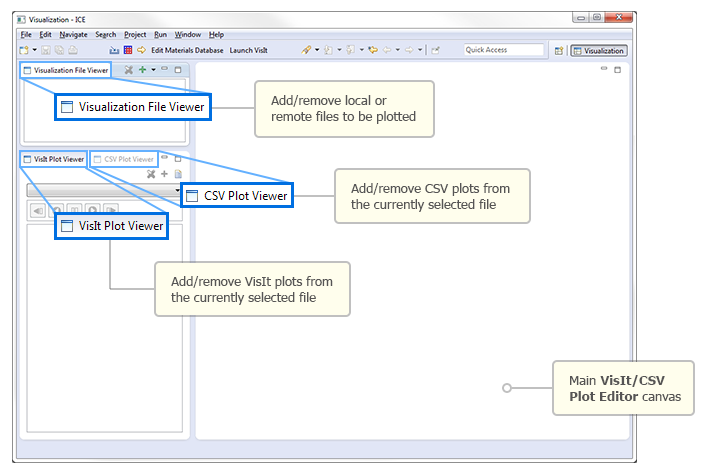
\includegraphics[width=\textwidth]{figures/ICE_VisualizationPerspective.png}
\caption{The ICE Visualization Perspective.}
\end{figure}

\section{Visualizing Output}\label{visualizing-output}

\subsection{VisIt}\label{visit}

\paragraph{Connecting to VisIt}\label{connecting-to-visit}

Once you switch to the \emph{Visualization Perspective}, the first step
necessary is to connect to your VisIt installation through ICE. To do
this, click on the \emph{Launch VisIt} button located in the ICE toolbar
near the top.

\begin{figure}[htbp]
\centering
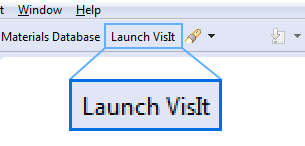
\includegraphics{figures/ICE_VisItLaunchButton.png}
\caption{The Launch VisIt button in the ICE toolbar.}
\end{figure}

A dialog will pop up offering you three options for connecting to VisIt:

\begin{figure}[htbp]
\centering
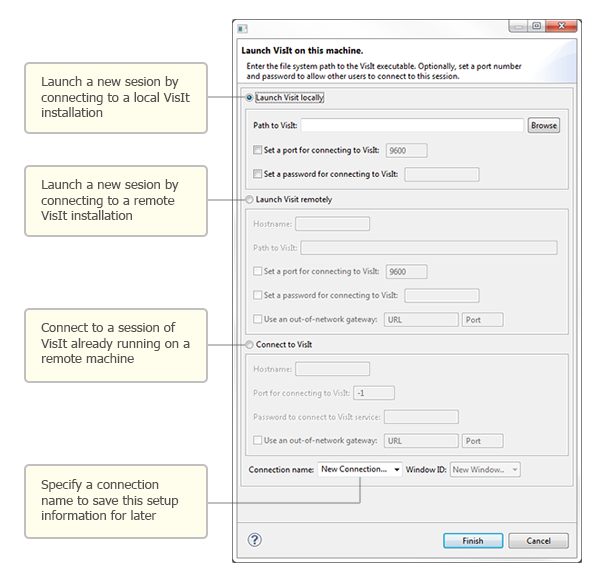
\includegraphics[width=\textwidth]{figures/ICE_VisItLaunchOptions.png}
\caption{The VisIt connection wizard in ICE.}
\end{figure}

\begin{enumerate}
\itemsep1pt\parskip0pt\parsep0pt
\item
  \textbf{Launch VisIt locally}\\If you installed VisIt on your local
  machine, use the \emph{Browse} button to direct ICE to your local
  installation directory. Using this method of connecting will launch a
  new VisIt session. Optionally, you can also set a port number (default
  9600) and-\/-if you want to share your VisIt session with another
  user-\/-a password.
\item
  \textbf{Launch VisIt remotely}\\If you installed VisIt on a remote
  machine, specify the hostname and full path to the VisIt installation
  directory. Using this method of connecting will launch a new VisIt
  session. Optionally, you can specify a port number (default 9600)
  and-\/-if you want to share your VisIt session with another user-\/-a
  password. If you need or want to use an external gateway or proxy to
  access the remote VisIt installation, you may specify its URL and port
  number as well.
\item
  \textbf{Connect to VisIt}\\If you would like to connect to session of
  VisIt already running somewhere else, specify the hostname, port
  number, and password set on the VisIt session; you will need to obtain
  this information from the person who initially launched the VisIt
  session. If you need or want to use an external gateway or proxy to
  access the remote VisIt installation, you may specify its URL and port
  number as well.
\end{enumerate}

Regardless of which method you choose to connect to VisIt, enter a
\emph{Connection name} at the bottom of the pop-up dialog. This will
allow you to re-use this connection information in the future.

If you are connecting to an existing session, specify a \emph{Window ID}
between 1 and 16. Which \emph{Window ID} you use depends on how you
would like to connect to VisIt. If multiple users connect using the same
\emph{Window ID}, they will all see and be able to interact with the
same VisIt view. However, if you would like multiple users to each have
their own unique session each with its own controls, assign a unique
\emph{Window ID} to each user. The VisIt installation can support up to
16 unique window IDs at a time.

Once you are done, click the \emph{Finish} button at the bottom, and ICE
should begin connecting to VisIt.

\paragraph{Adding/Removing Files}\label{addingremoving-files}

To open a file, find the green + icon in the \emph{Visualization File
Viewer}. Clicking directly on the green + icon will prompt a local
file browser to pop up. However, if your file is located on a remote
machine, or if you would like to add a file set, click on the drop-down
button next to the green + icon.

\begin{figure}[htbp]
\centering
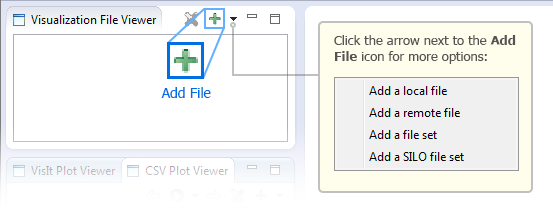
\includegraphics[width=\textwidth]{figures/ICE_VisItAddFileButton.png}
\caption{To add a new file to view in VisIt, click the green Add File button in the Visualization File View toolbar.}
\end{figure}

This will offer you four ways to open file(s):

\begin{itemize}
\itemsep1pt\parskip0pt\parsep0pt
\item
  Open a local file
\item
  Open a remote file
\item
  Open a local file set
\item
  Open a local SILO set
\end{itemize}

Once you have selected your file(s), they should appear in the
\emph{Visualization File Viewer}.

Lastly, if you would like to remove a file from the \emph{Visualization
File Viewer} list, select it, and click the red ``X'' button.

\paragraph{Adding/Removing Plots}\label{addingremoving-plots}

To begin adding plots, select your file in the \emph{Visualization File
Viewer} and click the green + icon in the \emph{VisIt Plot Viewer}.

\begin{figure}[htbp]
\centering
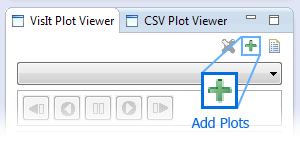
\includegraphics{figures/ICE_VisItAddPlotButton.png}
\caption{To add a new plot, click the Add Plots button in the VisIt Plot Viewer toolbar. }
\end{figure}

If there is any plottable data in your file, a dialog will pop up with a
list of options to choose from. This can include mesh plots, scalar
plots, vector plots, material block plots, and so forth. If there are
multiple plots of each type available, you can select them all by
checking off the entire category, or expand it to check off only
selected plots.

\begin{figure}[htbp]
\centering
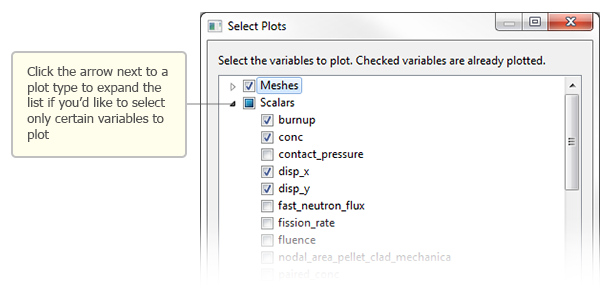
\includegraphics[width=\textwidth]{figures/ICE_VisItPlotSelection.png}
\caption{ICE prompts you with a list of available plots to select from. }
\end{figure}

When you are done selecting your plot(s), click \emph{OK}. The selected
plots should be added to the list in the \emph{VisIt Plot Viewer}.

Lastly, if you would like to remove a plot from the \emph{VisIt Plot
Viewer} list, select it and click the red ``X'' button.

\paragraph{Rendering Plots}\label{rendering-plots}

To render a plot, \emph{double} click it in the \emph{VisIt Plot
Viewer}, and it will appear in the main \emph{VisIt Editor}.

The \emph{VisIt Plot Viewer} contains a drop-down menu with a list of
plotting styles available for the currently selected plot. Depending on
your selected plot, this can include mesh, pseudo-color, contour,
volume, and so forth. Use this drop-down menu to select the plotting
style you prefer, and the \emph{VisIt Editor} will update in real time.

\begin{figure}[htbp]
\centering
\includegraphics{figures/ICE_VisItPlotStyleMenu.png}
\caption{You can select the plot type in the VisIt Plot Viewer drop-down menu.}
\end{figure}

The \emph{VisIt Editor} is also interactive in that you can move your
plot around by clicking and dragging the canvas or zoom by using the
mouse wheel. This may not necessarily be useful for 2D plots but enables
a fully rotatable look at 3D plots as in the example below.

\begin{figure}[htbp]
\centering
\includegraphics[width=\textwidth]{figures/ICE_VisIt3DNoise.png}
\caption{A view of a sample plot in the Visit Editor.}
\end{figure}

Lastly, if there is any time series data associated to your plot, you
can manually walk through the time steps, or play them continuously as a
short video, using the playback buttons located in the \emph{VisIt Plot
Viewer}.

\begin{figure}[htbp]
\centering
\includegraphics[scale=.6]{figures/ICE_VisItPlaybackButtons.png}
\caption{For time-series data, you can play through all time steps with the playback buttons in the Visit Plot Viewer. }
\end{figure}

\paragraph{Executing Python Commands}\label{executing-python-commands}

While many of VisIt's features are already accessible in ICE, work to
enable a more robust feature set is on-going. In the meantime, features
not yet integrated into ICE can still be accessed via Python commands by
clicking the Python script button located in the \emph{VisIt Plot
Viewer}.

\begin{figure}[htbp]
\centering
\includegraphics[scale=.6]{figures/ICE_VisItPythonScriptButton.png}
\caption{You can manipulate a VisIt plot with Python commands using the Execute Python Script button in the VisIt Plot Viewer.}
\end{figure}

Writing Python scripts for VisIt is beyond the scope of this tutorial.
However, you are welcome to refer to the
\href{https://wci.llnl.gov/simulation/computer-codes/visit/manuals}{VisIt
Python Interface Manual} provided by the VisIt development team at
Lawrence Livermore National Laboratory.

\subsubsection{CSV Plot Viewer}\label{csv-plot-viewer}

ICE includes, out of the box, basic CSV data plotting utilities for fast
and easy x/y graph visualizations. This section describes how to open
your CSV data using the \emph{CSV Plot Viewer} in the
\emph{\hyperref[Visualizationux5fPerspective]{Visualization
Perspective}}.

\paragraph{Adding/Removing Files}\label{addingremoving-files-1}

To open a file, find the green + icon in the \emph{Visualization File
Viewer}. Clicking directly on the green + icon will prompt a local
file browser to pop up. You can also access this option by clicking on
the drop-down button next to the green + icon.

\begin{figure}[htbp]
\centering
\includegraphics[width=\textwidth]{figures/ICE_VisItAddFileButton.png}
\caption{The VisIt Add File sub-menu.}
\end{figure}

This will offer you four ways to open file(s):

\begin{itemize}
\itemsep1pt\parskip0pt\parsep0pt
\item
  Open a local file
\item
  Open a remote file
\item
  Open a local file set
\item
  Open a local SILO set
\end{itemize}

Once you have selected your file(s), they should appear in the
\emph{Visualization File Viewer}.

Lastly, if you would like to remove a file from the \emph{Visualization
File Viewer} list, select it, and click the red ``X'' button.

\paragraph{Adding/Removing Plots}\label{addingremoving-plots-1}

\subparagraph{Adding Plots}\label{adding-plots}

To begin adding plots, select your file in the \emph{Visualization File
Viewer} and click the green + icon in the \emph{CSV Plot Viewer}.

\begin{figure}[htbp]
\centering
\includegraphics[width=\textwidth]{figures/ICE_CSVAddPlotButton.png}
\caption{The CSV Add Plot button.}
\end{figure}

\subparagraph{Selecting Initial Plot
Data}\label{selecting-initial-plot-data}

If the data in your CSV file is properly formatted, then a dialog will
appear. This dialog gives you a list of variables from your data file.

\begin{figure}[htbp]
\centering
\includegraphics[width=\textwidth]{figures/ICE_CSVAddPlotDialog-XAxisVariables.png}
\caption{The CSV Add Plot independent variables dialog. }
\end{figure}

In this first dialog, you select independent variables from your CSV
file. Independent variables are those whose values determine the
x-coordinates of plotted series. You can select multiple data as
independent variables by holding the \emph{CTRL} key while clicking
values in the dialog's list. When you are finished selecting independent
variables from the list, click \emph{OK} or press \emph{Enter}.

A second dialog allowing you to select the plot type will appear. The
default plot type is \emph{Line}, which when used means the
xy-coordinates of added series will be connected by a line. The plot
type selected from this dialog will be used for all series generated
from this sequence of dialogs.

\begin{figure}[htbp]
\centering
\includegraphics[scale=.6]{figures/ICE_CSVAddPlotDialog-PlotTypes.png}
\caption{The CSV plot type dialog.}
\end{figure}

Once you have chosen your desired plot type, click \emph{OK} or press
\emph{Enter}.

A third dialog allowing you to select the features that will actually be
plotted will appear.

\begin{figure}[htbp]
\centering
\includegraphics[width=\textwidth]{figures/ICE_CSVAddPlotDialog-Features.png}
\caption{ The CSV Plot features dialog.  }
\end{figure}

The list on the left includes the \emph{independent variables} selected
in one of the previous dialogs. You must select at least one of these
independent variables, as they provide the \emph{x}-coordinates of
series generated from the dialog.

The list on the right includes all \emph{features} available in the
file. You must select at least one of these features, as they provide
the \emph{y}-coordinates of series generated from the dialog.

You can also select multiple variables from either list by holding the
\emph{CTRL} key while clicking variables, although you should note that
every combination of selected independent (x) and feature (y) variables
will be plotted.

Once you have selected your desired x- and y-axis variables, click
\emph{OK} or press \emph{Enter}. A new plot will be added to the list in
the \emph{CSV Plot Viewer}. To open this plot, simply click it, and it
will open in a new \emph{CSV Plot Editor}.

\begin{figure}[htbp]
\centering
\includegraphics[width=\textwidth]{figures/ICE_CSVPlotEditor.png}
\caption{The ICE CSV Plot Editor. }
\end{figure}

\subparagraph{Showing/Moving Plots}\label{showingmoving-plots}

To re-open an existing plot, click its item in the \emph{CSV Plot
Viewer}, which is usually located on the left. The associated \emph{CSV
Plot Editor} in the main workbench space will be brought to the top or
activated. You can also click on the associated \emph{CSV Plot Editor}'s
tab to open it, or you can click and drag its tab to move it to another
spot in your workbench.

\begin{figure}[htbp]
\centering
\includegraphics[width=\textwidth]{figures/ICE_CSVPlotEditor-Moved.png}
\caption{You can move multiple plots around through mouse-click and drag.}
\end{figure}

\subparagraph{Removing Plots}\label{removing-plots}

Lastly, if you would like to remove a plot from the \emph{CSV Plot
Viewer} list, select it and click the red ``X'' button. To permanently
remove it from view, you will also need to close the \emph{CSV Plot
Editor} in the main workbench space.

\paragraph{Adding Series to a Plot}\label{adding-series-to-a-plot}

To add more series to an existing \emph{CSV Plot Editor}, you must first
select the desired plot in the \emph{CSV Plot Viewer}. Locate the green
+ button in the \emph{CSV Plot Viewer} and click on the drop-down
button next to it. Select \emph{Add a series}.

You will then be prompted with the same sequence of dialogs as in the
section on \hyperref[Selectingux5fInitialux5fPlotux5fData]{Selecting
Initial Plot Data}.

When you have finished selecting plot data as described in that section,
the new data will be added to your selected plot as new series.

\paragraph{Plot Toolbar}\label{plot-toolbar}

The plotting widget used by ICE's \emph{CSV Plot Editor} includes a
toolbar with helpful utilities for navigating your plotted data or
customizing the plot's appearance. You can hover the mouse cursor over
each button to view a tool tip describing what the button does.

Clicking the first button will open a dialog that allows you to
customize the appearance of the plot or individual series on the plot,
including titles, scales, grids, colors, and fonts. The last button
allows you to save the current appearance of the plot to a \texttt{.png}
image file. Feel free to try out the different utilities available in
this toolbar.

\chapter{Developing MOOSE Applications with ICE}
\label{sec:devMoose}

\section{Introduction}\label{introduction}

This article is designed to walk MOOSE developers through a typical
workflow for developing MOOSE-based applications in ICE. Since ICE is
built on top of the Eclipse platform, a large variety of sophisticated
software development tools and technologies for developing scientific
software can be integrated into the ICE platform. Version control, code
editing, code completion, code building, and code generation are just a
few of the various technologies now available to MOOSE-based application
developers using ICE. Additionally, after developing your custom MOOSE
application, the usual MOOSELauncher and MOOSEModel Items and the ICE
Visualization perspective are still at your disposal for constructing
input files, launching jobs, and visualizing results.

\section{Cloning MOOSE}\label{cloning-moose}

To clone MOOSE, simply switch to the Git Perspective in the top right
corner of ICE. You will be presented with the following view.

\begin{figure}[htbp]
\centering
\includegraphics[width=\textwidth]{figures/GitView.png}
\caption{A view of the ICE Git Perspective.}
\end{figure}

Now click the 'Clone a Git Repository' button in the toolbar of the 'Git
Repository' view (or the hyperlink in the middle of the view if you have
not repositories). You will be presented with the following wizard.

\begin{figure}[htbp]
\centering
\includegraphics[width=\textwidth]{figures/Clone_wizard.png}
\caption{The first page of the Clone Repository Wizard requesting information about the remote Git repository URL.}
\end{figure}
\begin{figure}[htbp]
\centering
\includegraphics[width=\textwidth]{figures/Clone_wizard2.png}
\caption{The second page of the Clone Repository Wizard requesting information about which branches to pull down.}
\end{figure}
\begin{figure}[htbp]
\centering
\includegraphics[width=\textwidth]{figures/Clone_wizard3.png}
\caption{The final page of the Clone Repository Wizard requesting information about the local location of the repository.}
\end{figure}

Enter \url{https://github.com/idaholab/moose} into the URI entry and
select next. This will present you with the branch selection wizard
page. Select which branches you'd like to import in this clone and click
Next. The last page will let you specify the clone location on your
local filesystem. If you'd like this to be in your local ICE workspace
entry /home/username/ICEFiles in the entry and click Finish.

To import MOOSE into your ICE Project Explorer, simply right click the
created moose repository in the Git Repository view and select 'Import
Projects'. On the first wizard page, select 'Import as New Project' and
click finish. This will present you with the ICE New Project wizard. In
this wizard, open the C/C++ tree node and select 'Makefile project with
Existing Code'. Provide a valid project name and toolchain and click
finish. You should see MOOSE in your Project Explorer.

\begin{figure}[htbp]
\centering
\includegraphics[width=\textwidth]{figures/Import_git_proj.png}
\caption{The import projects wizard for the ICE Git repositories view. }
\end{figure}

\section{Building MOOSE}\label{building-moose}

To build MOOSE/Libmesh within ICE, open the Make Target view by going to
Window \textgreater{} Show View \textgreater{} Other and search and
select Make Target. With MOOSE imported into your Project Explorer, you
should see the MOOSE project in the Make Target view. Right click on
that project and select New. A dialog will pop up prompting you for the
Make Target name, target name, and build command. Set the name as 'Build
Libmesh', uncheck 'Same as target name' and leave the Make target blank,
uncheck 'Use builder settings' and set the command as 'sh
scripts/update\_and\_rebuild\_libmesh.sh', then click 'Ok'. Now you
should see a 'Build Libmesh' target, which upon double-clicking will
execute the update\_and\_rebuild\_libmesh.sh script with the output
streaming in the Console view.

Once that is done, you can create another Make Target in the same
manner, this time setting the target as all, but setting the build
command (assuming you have CMake installed on your system) as 'cmake -E
chdir framework make' (feel free to add -j N to this command, where N is
the number of make threads). If you do not have CMake installed, you can
right click on the MOOSE project in the Project Explorer and select
Properties. In this Properties dialog, select C/C++ Build and append to
the Build directory entry 'framework'. Now, double-clicking this make
target will execute the MOOSE build, and you should see the output
streaming in the Console.

\section{Forking the Stork}\label{forking-the-stork}

The internal MOOSE development team provides another GitHub repository
called stork at \url{https://github.com/idaholab/stork} that represents
the base structure needed to create a new MOOSE application. So 'Forking
the Stork' implies forking this repository, changing its name to
whatever you've decided to call your MOOSE application, and cloning that
locally to begin work. The MOOSE team calls this 'Forking the Stork' and
provides a link to the repository at mooseframework.org/create-an-app.

ICE now provides this functionality in an easy-to-use toolbar button
using the tools provided by the Eclipse EGit plugins. To 'Fork the
Stork' in ICE, simply click the 'MOOSE Fork the Stork' button in the
toolbar.

\begin{figure}[htbp]
\centering
\includegraphics[width=\textwidth]{figures/Fork_button.png}
\caption{The ICE Fork the Stork button in the toolbar. }
\end{figure}
\begin{figure}[htbp]
\centering
\includegraphics[width=\textwidth]{figures/Fork_dialog.png}
\caption{The Fork the Stork Wizard for entering your new MOOSE application name and your GitHub credentials.}
\end{figure}

This will present a new dialog asking for the name of your new MOOSE
application, as well as your GitHub username and password. Upon
providing this information and clicking 'Ok', ICE will fork the
\url{https://github.com/idaholab/stork} repository for you, rename it to
your provided application name, clone it to \textasciitilde{}/ICEFiles,
and import it into ICE as a new C++ project in the C/C++ perspective's
Project Explorer view.

Additionally, the import generates a fully configured Make Target in the
Make Target view, and sets up the C++ Indexer to point to your ICE MOOSE
project's include files. This is essential for providing code completion
and MOOSE code search while your developing your MOOSE application. To
look at a MOOSE class that you've referenced in one of your
application's source files, simply click the class name or the header
file and click F3. ICE will take you directly to the declaration for
that MOOSE class so that you can peruse and look up its method
definitions.

\begin{figure}[htbp]
\centering
\includegraphics[width=\textwidth]{figures/New_app.png}
\caption{ICE creates the newly forked MOOSE application as a C/C++ project in the Project Explorer.}
\end{figure}
\begin{figure}[htbp]
\centering
\includegraphics[width=\textwidth]{figures/Make_target.png}
\caption{ICE adds a new Make Target to the Make Targets View for building your new application.}
\end{figure}

\newpage

\section{Adding a New Kernel}\label{adding-a-new-kernel}

Once you've cloned and built MOOSE, and Forked the Stork to produce a
new MOOSE application ready for development, you can easily create
custom Kernels with ICE. To create a new Kernel, right click on your new
MOOSE-based application project and select New \textgreater{} MOOSE
Object \textgreater{} Kernel.

\begin{figure}[htbp]
\centering
\includegraphics[width=\textwidth]{figures/New_kernel.png}
\caption{Creating a new Kernel in ICE is easy, just right click on your project and select New - MOOSE Object - Kernel.}
\end{figure}

This action will display an input prompt asking for the name of your new
Kernel subclass. Simply enter the name and push 'Ok'. Then ICE will
automatically generate a new include and source file in include/kernel
and source/kernel, respectively. The new files are the stubbed out, base
implementation of a subclassed Kernel that you can then add to and
modify.

\begin{figure}[htbp]
\centering
\includegraphics[width=\textwidth]{figures/Kernel_source.png}
\caption{The created source code for the Add Kernel context menu action. }
\end{figure}

\section{Building your MOOSE App}\label{building-your-moose-app}

Building your MOOSE application is simple because the 'Fork the Stork'
action produced a Make Target for you. Simply double-click that make
target and you application will build, producing the application
executable.

\section{Pushing Changes Back to
GitHub}\label{pushing-changes-back-to-github}

To push changes to the remote GitHub repository at
\url{https://github.com/username/animal}, switch back to the Git
perspective and click your applications git repository in the Git
Repositories view. On the bottom right of the screen, you should see
another set of tabbed views, one of them being the Git Staging view.

\begin{figure}[htbp]
\centering
\includegraphics[width=\textwidth]{figures/Git_commit.png}
\caption{Committing your new MOOSE application is easy, just stage it in the Git Staging view of the Git Repositories Perspective.}
\end{figure}

Click the Git Staging View and drag any Unstaged Changes to the Staged
Changes section. Now provide a brief commit message and click 'Commit
and Push', enter your GitHub credentials, and watch as your files are
committed to the remote repository!

\section{Executing Built MOOSE
Application}\label{executing-built-moose-application}

Now that you've developed a new MOOSE application you need to develop
input files for it and execute it to see your desired results. This is
simple with ICE: just use the built in MOOSE Model Builder and MOOSE
Launcher Items. Detailed instructions can be found at
\href{Using MOOSE with ICE}{Using MOOSE with ICE}.


\renewcommand{\bibname}{Online Resources}
\nocite{*}
\bibliographystyle{plain}
\bibliography{sections/mainBib}
%\input{sections/biblio}
%\chapter{Online Resources}
\label{sec:resources}

ICE Wiki: \url{https://wiki.eclipse.org/ICE}

\noindent ICE Bugs: \url{https://bugs.eclipse.org/bugs/describecomponents.cgi?product=Ice}

\noindent VisIt: \url{https://wci.llnl.gov/simulation/computer-codes/visit/}

\noindent MOOSE: \url{https://mooseframework.org}

\noindent MOOSE GitHub: \url{https://github.com/idaholab/moose}

\noindent MOOSE Stork: \url{https://github.com/idaholab/stork}
%\input{availability}
%\input{tutorial}

\end{document}

